\chapter{Inserting and Deleting Rows}
\label{ch:rows}

\section{The commands}
\index{rows!inserting}\index{rows!deleting}

\begin{cctable}{Command}{Effect}{2.2in}{2.62in}
\menupath{Layout > Insert row} & Opens a blank row above the cursor's row,
pushing everything below it down one \\
\menupath{Layout > Delete row} & Removes the cursor's row, pulling everything
below it up one \\
\end{cctable}

Both act on the whole row, across every column that is in use, on the current
worksheet only. Neither has a keyboard shortcut.

\section{Inserting}

Put the cursor anywhere on the row you want the new row to appear \emph{above},
and choose \menupath{Layout > Insert row}.

There is no confirmation. The row appears immediately.

Inserting does nothing if the worksheet is empty, or if the cursor is below the
last row in use --- there is nothing there to push down. It fails if the last
row in use is already row 65,534, because there would be nowhere for the bottom
row to go.

\section{Deleting}

Put the cursor on the row and choose \menupath{Layout > Delete row}. \ccprod{}
asks first, on the bottom line of the screen:

\begin{ccfigure}
\ccscreenscale{1.5}
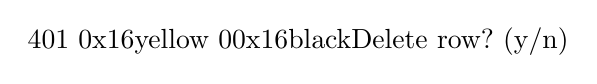
\begin{tikzpicture}
\node[inner sep=0pt,anchor=north west] (dr) at (0,0) {%
\ccscreenbegin{40}{1}
  \ccfillrow{0}{x16yellow}
  \cctext{0}{0}{x16black}{Delete~row?~(y/n)}
\ccscreenend
};
\end{tikzpicture}
\caption{The delete-row question, on the message line}
\label{fig:delrow}
\end{ccfigure}

\key{Y} deletes the row. Any other key leaves it alone.

\begin{cccaution}
There is no undo. \key{F5} restores one cell, not one row, and it has no record
of a row that has been removed. The question on the message line is the only
protection there is.
\end{cccaution}

\section{What happens to formulas}
\index{formulas!adjusted on insert and delete}

Inserting or deleting a row rewrites the references inside every formula in the
worksheet so that they go on meaning the same cells.

\begin{ccexamples}[Insert a row above row 5]{0.44\linewidth}
\exn{=SUM(B2:B9)}{=SUM(B2:B10)}{the range grows}
\exn{=B7*2}{=B8*2}{the reference follows its cell}
\exn{=B2+B3}{=B2+B3}{above the cut: unchanged}
\end{ccexamples}

\begin{ccexamples}[Delete row 5]{0.44\linewidth}
\exn{=SUM(B2:B9)}{=SUM(B2:B8)}{the range shrinks}
\exn{=B7*2}{=B6*2}{}
\end{ccexamples}

Ranges come out right whether the row was inside them or was one of their
corners. A \lit{\$} in a reference makes no difference and is not meant to: a
dollar sign fixes a reference against \emph{copying}, and a row that has
physically moved has moved for everybody.

The rewrite happens before the recalculation, so the numbers you see afterwards
are already the corrected ones.

\subsection{Three cases it does not cover}

\begin{cccaution}
\textbf{A reference that names another worksheet is left alone.} \fml{=Sheet2!A1}
still says \cellref{A1} after a row is inserted on \emph{Sheet2}. Inserting or
deleting rows on a worksheet that others read from means checking those others
by hand.

\textbf{Deleting the row a formula points straight at} leaves the formula
pointing at that row number, which now holds whatever moved up into it.
Excel would put \errv{\#REF!} there; \ccprod{} cannot, because the corrected
formula goes back through the compiler and there is no way to write
\errv{\#REF!} that the compiler will accept. The formula keeps working and
quietly reads the wrong row.

\textbf{A formula longer than 128 characters is skipped entirely} and keeps its
original references. Rewriting it safely needs more working space than the
program has, and a formula truncated half way through is worse than one that
did not move.
\end{cccaution}

\subsection{What still does not adjust}

\begin{cccaution}
Two things are left alone wherever a formula moves, and both are deliberate.

\textbf{A reference naming another worksheet} --- \fml{Q1!B5} --- is never
rewritten. Inserting a row on this sheet does not move a reference pointing at
that one.

\textbf{A formula longer than 128 characters} is skipped whole rather than
half-rewritten. The rewriter works on the source text and has one buffer for
it; a formula truncated part way through would be worse than one that did not
move.
\end{cccaution}

\begin{ccnote}
Deleting the row a formula points at does not produce \msg{\#REF!}. The
reference is left pointing at that row number, which now holds whatever moved
up into it. Check formulas that referred to a row you have deleted.
\end{ccnote}

\section{What these commands do not do}

There is no way to insert or delete a single cell and shift its neighbours, and
no way to insert or delete more than one row or column at a time --- to open
five rows, run \menupath{Insert row} five times.
